%% abtex2-modelo-artigo.tex, v-1.9.6 laurocesar
%% Copyright 2012-2016 by abnTeX2 group at http://www.abntex.net.br/ 
%%
%% This work may be distributed and/or modified under the
%% conditions of the LaTeX Project Public License, either version 1.3
%% of this license or (at your option) any later version.
%% The latest version of this license is in
%%   http://www.latex-project.org/lppl.txt
%% and version 1.3 or later is part of all distributions of LaTeX
%% version 2005/12/01 or later.
%%
%% This work has the LPPL maintenance status `maintained'.
%% 
%% The Current Maintainer of this work is the abnTeX2 team, led
%% by Lauro César Araujo. Further information are available on 
%% http://www.abntex.net.br/
%%
%% This work consists of the files abntex2-modelo-artigo.tex and
%% abntex2-modelo-references.bib
%%

% ------------------------------------------------------------------------
% ------------------------------------------------------------------------
% abnTeX2: Modelo de Artigo Acadêmico em conformidade com
% ABNT NBR 6022:2003: Informação e documentação - Artigo em publicação 
% periódica científica impressa - Apresentação
% ------------------------------------------------------------------------
% ------------------------------------------------------------------------

\documentclass[
	% -- opções da classe memoir --
	article,			% indica que é um artigo acadêmico
	11pt,				% tamanho da fonte
	oneside,			% para impressão apenas no recto. Oposto a twoside
	a4paper,			% tamanho do papel. 
	% -- opções da classe abntex2 --
	%chapter=TITLE,		% títulos de capítulos convertidos em letras maiúsculas
	%section=TITLE,		% títulos de seções convertidos em letras maiúsculas
	%subsection=TITLE,	% títulos de subseções convertidos em letras maiúsculas
	%subsubsection=TITLE % títulos de subsubseções convertidos em letras maiúsculas
	% -- opções do pacote babel --
	english,			% idioma adicional para hifenização
	brazil,				% o último idioma é o principal do documento
	sumario=tradicional
	]{abntex2}


% ---
% PACOTES
% ---

% ---
% Pacotes fundamentais 
% ---
\usepackage{lmodern}			% Usa a fonte Latin Modern
\usepackage[T1]{fontenc}		% Selecao de codigos de fonte.
\usepackage[utf8]{inputenc}		% Codificacao do documento (conversão automática dos acentos)
\usepackage{indentfirst}		% Indenta o primeiro parágrafo de cada seção.
\usepackage{nomencl} 			% Lista de simbolos
\usepackage{color}				% Controle das cores
\usepackage{graphicx}			% Inclusão de gráficos
\usepackage{microtype} 			% para melhorias de justificação
% ---
		
% ---
% Pacotes adicionais, usados apenas no âmbito do Modelo Canônico do abnteX2
% ---
\usepackage{lipsum}				% para geração de dummy text

\usepackage[        %algoritmos
    boxruled,           %caixa em volta
    linesnumbered,    %numeração das linhas
    portuguese        %para algoritmos em portuguese
    ]{algorithm2e}
% ---
		
% ---
% Pacotes de citações
% ---
\usepackage[brazilian,hyperpageref]{backref}	 % Paginas com as citações na bibl
\usepackage[alf]{abntex2cite}	% Citações padrão ABNT
% ---

% ---
% Configurações do pacote backref
% Usado sem a opção hyperpageref de backref
\renewcommand{\backrefpagesname}{Citado na(s) página(s):~}
% Texto padrão antes do número das páginas
\renewcommand{\backref}{}
% Define os textos da citação
\renewcommand*{\backrefalt}[4]{
	\ifcase #1 %
		Nenhuma citação no texto.%
	\or
		Citado na página #2.%
	\else
		Citado #1 vezes nas páginas #2.%
	\fi}%
% ---

% ---
% Informações de dados para CAPA e FOLHA DE ROSTO
% ---
\titulo{Trabalho 1 - parte 1\\ INE5430 - Inteligência Artificial}
\autor{Bruno Marques do Nascimento{\thanks{brunomn95@gmail.com}} \and
       Johann Westphall \thanks{johannwestphall@gmail.com}}
\local{Brasil}
\data{Florianópolis, 22 de Agosto de 2017}
% ---

% ---
% Configurações de aparência do PDF final

% alterando o aspecto da cor azul
\definecolor{blue}{RGB}{41,5,195}

% informações do PDF
\makeatletter
\hypersetup{
     	%pagebackref=true,
		pdftitle={\@title}, 
		pdfauthor={\@author},
    	pdfsubject={Modelo de artigo científico com abnTeX2},
	    pdfcreator={LaTeX with abnTeX2},
		pdfkeywords={abnt}{latex}{abntex}{abntex2}{atigo científico}, 
		colorlinks=true,       		% false: boxed links; true: colored links
    	linkcolor=blue,          	% color of internal links
    	citecolor=blue,        		% color of links to bibliography
    	filecolor=magenta,      		% color of file links
		urlcolor=blue,
		bookmarksdepth=4
}
\makeatother
% --- 

% ---
% compila o indice
% ---
\makeindex
% ---

% ---
% Altera as margens padrões
% ---
\setlrmarginsandblock{3cm}{3cm}{*}
\setulmarginsandblock{3cm}{3cm}{*}
\checkandfixthelayout
% ---

% --- 
% Espaçamentos entre linhas e parágrafos 
% --- 

% O tamanho do parágrafo é dado por:
\setlength{\parindent}{1.3cm}

% Controle do espaçamento entre um parágrafo e outro:
\setlength{\parskip}{0.2cm}  % tente também \onelineskip

% Espaçamento simples
\SingleSpacing

% ----
% Início do documento
% ----
\begin{document}

% Seleciona o idioma do documento (conforme pacotes do babel)
%\selectlanguage{english}
\selectlanguage{brazil}

% Retira espaço extra obsoleto entre as frases.
\frenchspacing 

% ----------------------------------------------------------
% ELEMENTOS PRÉ-TEXTUAIS
% ----------------------------------------------------------

%---
%
% Se desejar escrever o artigo em duas colunas, descomente a linha abaixo
% e a linha com o texto ``FIM DE ARTIGO EM DUAS COLUNAS''.
% \twocolumn[    		% INICIO DE ARTIGO EM DUAS COLUNAS
%
%---
% página de titulo
\maketitle

% ]  				% FIM DE ARTIGO EM DUAS COLUNAS
% ---

% ----------------------------------------------------------
% ELEMENTOS TEXTUAIS
% ----------------------------------------------------------
\textual

% ----------------------------------------------------------
% Introdução
% ----------------------------------------------------------
\section*{Introdução}
\addcontentsline{toc}{section}{Introdução}

Este relatório possui o objetivo de explicar o que foi desenvolvido para a primeira entrega do Trabalho 1 da disiciplina de Inteligência Artifical, ministrada pelo professor Elder Rizzon Santos na Universidade Federal de Santa Catarina(UFSC), campus Florianópolis.
O propósito do trabalho é implementar o algoritmo de busca adversária MiniMax com podas $\alpha$ e $\beta$. A implementação será testada através do jogo 5 em linha (Gomoku), com tabuleiro tamanho 15x15. 

Nesta primeira etapa, serão abordadas as definições matemáticas da função utilidade e heurística, e a implementação parcial da função heurística. Além disso, será explicado como são realizadas as detecções de fim de jogo e sequências de 4 peças. 

A linguagem de programação \textit{C++} foi a escolhida para a implementação do trabalho e para o desenvolvimento da interface gráfica a API gtkmm-3.0. 

% ----------------------------------------------------------
% Seção de explicações
% ----------------------------------------------------------
\section{Definições matemáticas}

\subsection{Utilidade}
\subsection{Heurística}


\begin{verbatim}
   \setlrmarginsandblock{3cm}{3cm}{*}
   \setulmarginsandblock{3cm}{3cm}{*}
   \checkandfixthelayout
\end{verbatim}

\section{Detecções}

\subsection{Fim de jogo}

Após cada jogada feita por qualquer jogador é verificado se o jogo acabou
a partir das coordenadas 'x' e 'y' da jogada. Considerando que uma sequência de vitória é formada
por 5 símbolos consecutivos em qualquer direção, uma solução seria buscar no tabuleiro inteiro por
essa sequência.

Todavia uma maneira mais eficiente de se fazer isso foi implementada. A partir do 'x' e 'y' da jogada, são extraídas as respectivas linhas, colunas e diagonais a qual esta jogada pertence, conforme \autoref{extracao_estruturas}. Após, é realizada a busca em cada uma das estruturas extraídas com o intuíto de achar uma sequência que conceda a vitória para um dos jogadores, que seria uma sequência ininterrupta de 5 símbolos iguais, petencentes ao mesmo jogador.

\begin{figure}[htb]
    \caption{\label{extracao_estruturas}Extração das estruturas pertencentes a jogada.}
        \begin{center}
            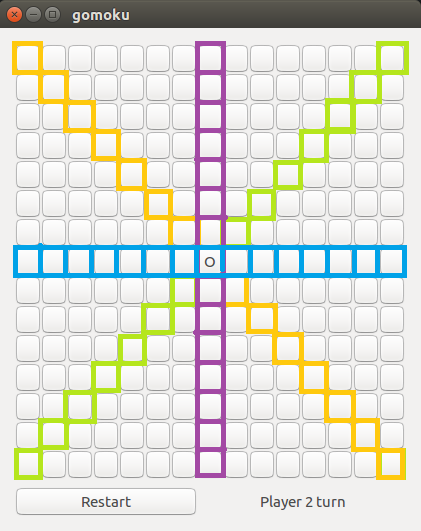
\includegraphics[scale=0.75]{busca_de_vitoria.png}
        \end{center}
\end{figure}

\subsection{Sequência de 4 símbolos}

A fim de detectar a sequência de 4  é aplicado o mesmo algoritmo para a detecção de fim de jogo, no qual a sequência buscada é de 5 símbolos, porém agora para um conjunto de 4 símbolos iguais consecutivos.

Foi verificado que esse método não detecta possibilidade com 'buracos' entre peças como, por exemplo na \autoref{nao_detecta}, e para a entrega final será implementado o algoritmo que verifica qualquer configuração de 4 símbolos que dê a possibilidade de vitória para um dos jogadores.

\begin{figure}[htb]
    \caption{\label{detecta}Sequência de 4 símbolos: detecta.}
        \begin{center}
            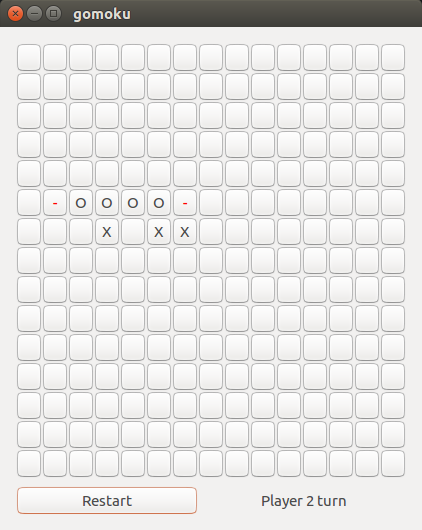
\includegraphics[scale=0.71]{detecta.png}
        \end{center}
\end{figure}

\begin{figure}[htb]
    \caption{\label{nao_detecta}Sequência de 4 símbolos: não detecta.}
        \begin{center}
            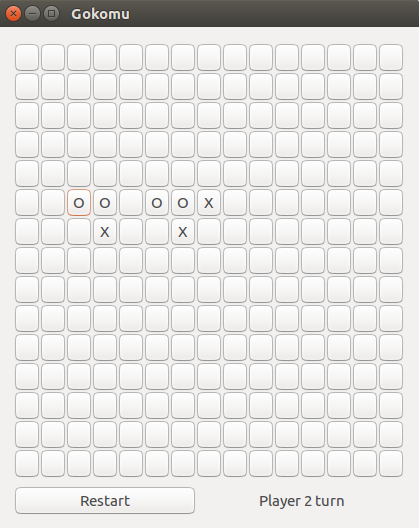
\includegraphics[scale=0.55]{naodetecta.png}
        \end{center}
\end{figure}

% ---
% Finaliza a parte no bookmark do PDF, para que se inicie o bookmark na raiz
% ---
\bookmarksetup{startatroot}% 
% ---

% ---
% Conclusão
% ---
% \section*{Considerações finais}
% \addcontentsline{toc}{section}{Considerações finais}

% ----------------------------------------------------------
% ELEMENTOS PÓS-TEXTUAIS
% ----------------------------------------------------------
\postextual

% ]  				% FIM DE ARTIGO EM DUAS COLUNAS
% ---

% ----------------------------------------------------------
% Referências bibliográficas
% ----------------------------------------------------------
\bibliography{abntex2-modelo-references}

% ----------------------------------------------------------
% Glossário
% ----------------------------------------------------------
%
% Há diversas soluções prontas para glossário em LaTeX. 
% Consulte o manual do abnTeX2 para obter sugestões.
%
%\glossary

% ----------------------------------------------------------
% Apêndices
% ----------------------------------------------------------


\end{document}